\documentclass{article}
\usepackage{fontspec}
\setmonofont[Ligatures=TeX,SizeFeatures={Size=8}]{Hack}
\usepackage{tabularx}
\usepackage{pdfpages}
\usepackage{hyperref}
\usepackage{dirtytalk}
\usepackage[margin=2.5cm]{geometry}
\usepackage{setspace}
\usepackage{silence}
\WarningsOff*

\usepackage{etoolbox}
\AtBeginEnvironment{quote}{\singlespacing\small}

\newcommand\Tstrut{\rule{0pt}{2.9ex}}         % "top" strut
\newcommand\Bstrut{\rule[-1.2ex]{0pt}{0pt}}   % "bottom" strut

\title{NSN Writeup}
\author{Linus Molteno}
\date{}

\begin{document}

\maketitle

\section{Database}

The database needs to be a production-quality bit of software that required minimal maintenance, and could be self-contained, but allowing access from outside. It also of course needs to be able to store the correct information needed for the end product, regarding the standards. This information was:
\begin{itemize}
    \item Standards:
        \begin{itemize}
            \item Standard Number
            \item Title
            \item Number of credits
            \item Level
            \item Version (where available)
            \item Internal/External
            \item Achievement/Unit
            \item Structure (Field, Subfield, Domain)
            \item Subject (Separate because NCEA vs NZQA classification of standard)
        \end{itemize}
\end{itemize}

\begin{figure}
    \fbox{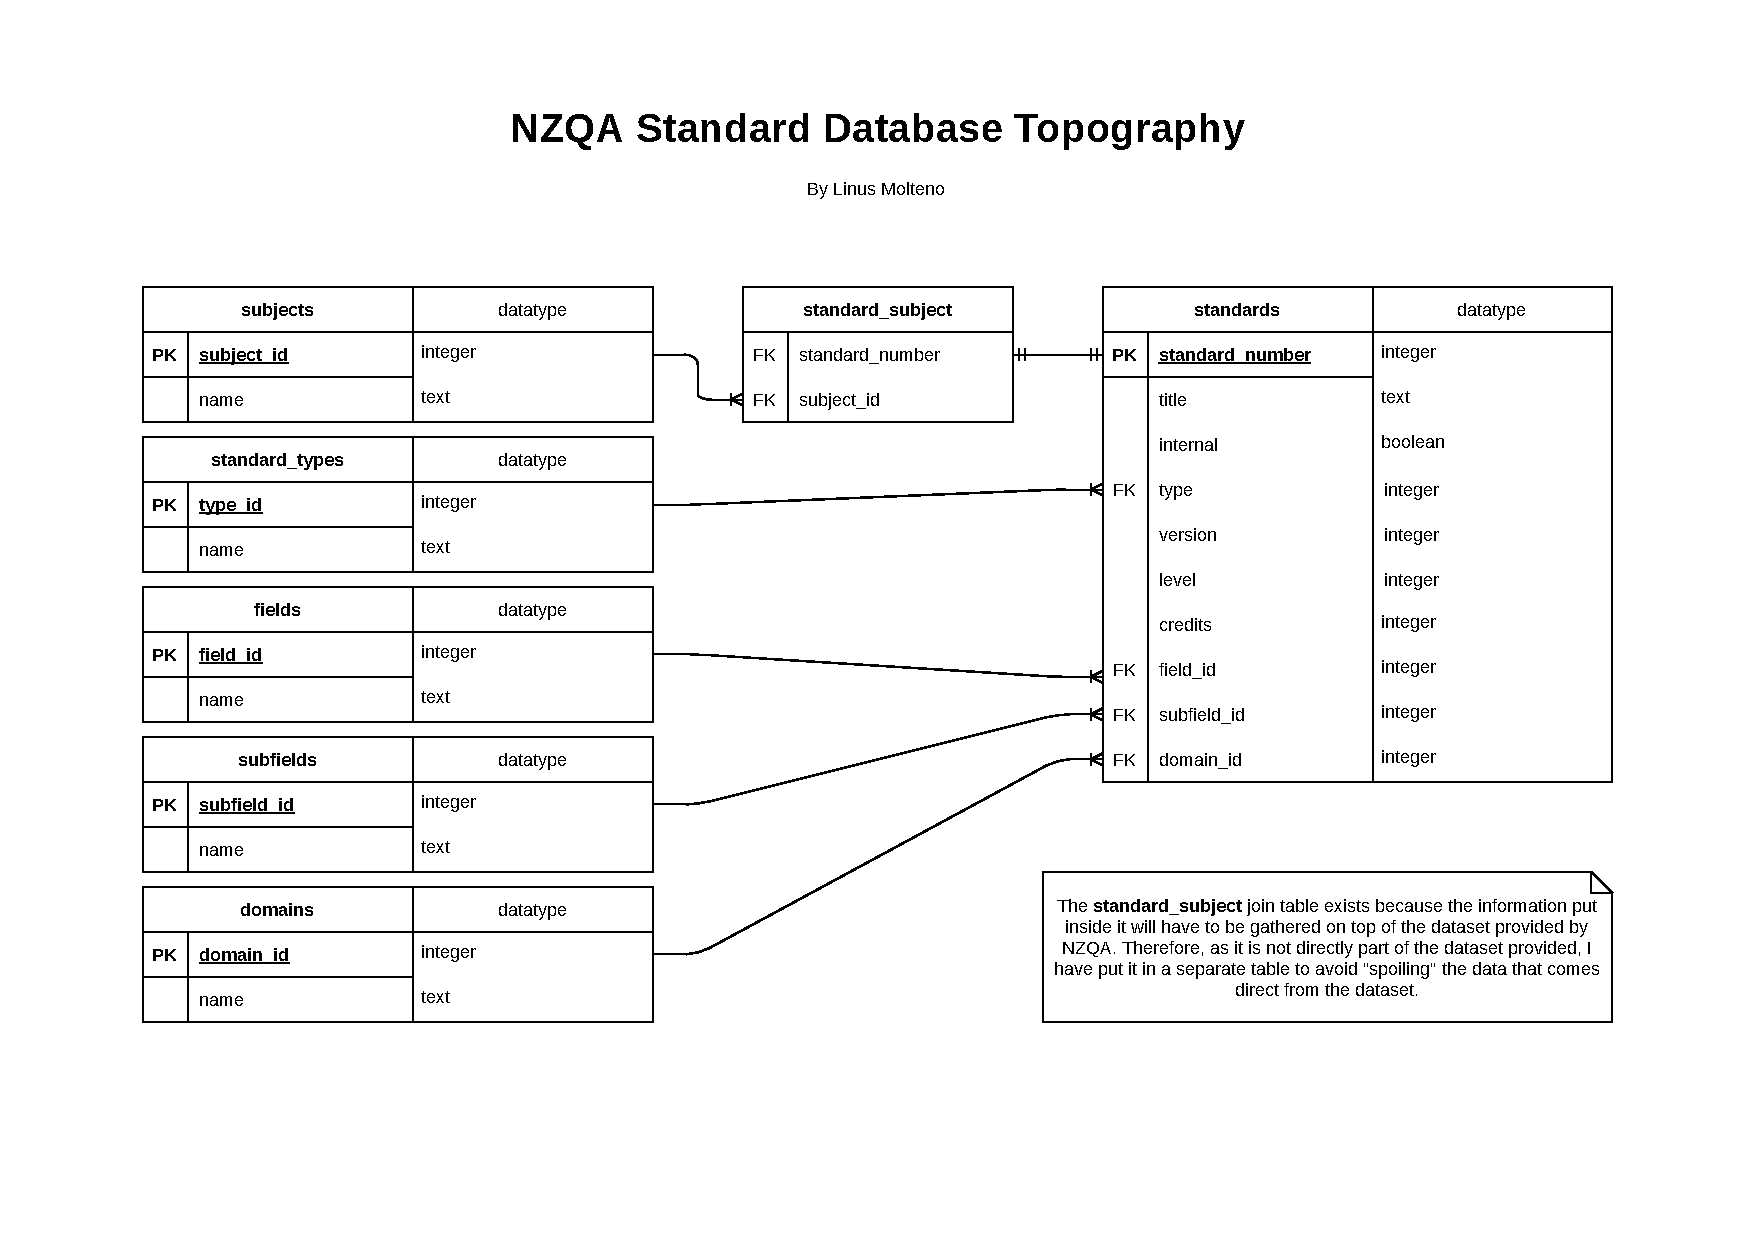
\includegraphics[page=1,width=\textwidth]{db.pdf}}
    \caption{Database topography, generated by \texttt{draw.io}. This is also available in the \texttt{github} repo. This was later changed as more features were added (e.g. resources, content)}
    \label{fig:dbtopography}
\end{figure}
The method in which I decided to approach the structured representation of this information in a database is represented in Figure~\ref{fig:dbtopography}.

\subsection*{Problem}
In the first stage of the waterfall development process, I had designed a system to take in the information from the NZQA-provided dataset of standards, and to enter them into a PostgreSQL database, as this was a production-quality form. However, it turned out that the NZQA-provided dataset didn’t give enough information for me to organise the standards as I wished. What I required was the NCEA (\textit{not NZQA}) subject that each standard was associated with. This was different to the classification system the NZQA dataset (field, subfield, domain), and I hate it.
\subsection*{Solution}
In order to get around this problem, I designed and implemented a python script (\texttt{ncea\_scraper.py}) that gathers the names of all the subjects, then scrapes each subject page to find the relevant assessments, and stores it in JSON format. In order to prevent it seeming like I'm DDoSing NZQA, I've added a random delay as well.
\subsubsection*{Commits}
\begin{description}\small
    \item[\texttt{f8fd2a2}] Began NZQA scraper for getting a list of all subjects
    \item[\texttt{9b4c0a6}] Finished NZQA scraper, will test on cloud instance for faster connection
    \item[\texttt{419f833}] Moved \texttt{nqza\_scraper} > \texttt{ncea\_scraper} because it's a more fitting name
    \item[\texttt{f065d95}] Ran NCEA scraper on google cloud instance for extra speed
\end{description}
\normalfont
\begin{center}
\rule{0.5\textwidth}{0.2pt}
\end{center}

\subsection*{Problem}
In testing encountered a whole lot of problems associated with getting PostgreSQL running, configuring users and connecting to it with Python.
\subsection*{Solution}
Revisiting the design stage, I've decided to put everything into Docker containers, as there is a simple Postgres container that would be easy to use. The use of containerisation allows setup to be easier for multiple different servers, as well as simple load-sharing further down the line. Doing this early also helps make that easier in the future as more is added. It is the best solution for a project with a lot of moving parts that might need to be moved to another machine, as VMs aren't dependent on the host hardware/software. The scraper is run in its own container, that checks whether the current data is out of date (1 year old). It also enters the data into the database.

\subsubsection*{Commits}
\begin{description}\small
    \item[\texttt{de3330a}] Began dockerisation, basic backend flask for testing, and fixed main.sql
    \item[\texttt{fc5bade0}] Moved to separate docker container for scraping/db entry
    \item[\texttt{f24617b}] Fixed bugs in \texttt{ncea\_scraper} regarding its inclusion as a docker container
\end{description}
\normalfont
\begin{center}
\rule{0.5\textwidth}{0.2pt}
\end{center}

\subsection*{Problem}
In testing with NZQA data, I encountered a problem where some of the titles didn't match between the dataset, and the scraped data. The reason for this seemed to be that the parsing software I used didn't handle accented characters (e.g. Te t\={u}hura i ng\={a} tuhinga raupeka) and replaced them with a ? (e.g. Te t?hura i ng? tuhinga raupeka). As well as this, there was a general mismatch, where the website had different titles in general, with different wording. Often this was more descriptive.
\subsection*{Solution}
Analysing the dataset, I found that the provided dataset just replaced these accented characters with characters without accents (\={a} goes to just a). This will provide a solution, as these characters are easier to handle down the line. Potential later enhancement would be handling and finding where the macrons should go. When the titles are valid but different, I'm choosing the website title, as these seem to be more descriptive. This could have been solved with more careful analysis before 

\subsubsection*{Commits}
\begin{description}\small
    \item[\texttt{8713b9e}] Finished combination of data with title mismatch handling, and null version handling
\end{description}
\normalfont

\begin{center}
\rule{0.5\textwidth}{0.2pt}
\end{center}

\subsection*{Problem}
When trying to run the scraping Docker container, I found that it kept rerunning the scrape and entering scripts, which is dumb, resource-wasteful, and unnecessary.
\subsection*{Solution}
This was because I had accidentally configured the default command for the container to be running those scripts, and when they were done running, it would restart the container, rerunning the commands. To fix this, I created a \texttt{checker.py} script that checks to see whether the scraped data is out of date every hour (if it it's out of date, re-scrape, clean db etc.), then set \textit{this} as the default command for the container. This way, this checker runs 24/7, and doesn't close the container, so no resources are wasted. I encountered a problem with the docker running the script when the \texttt{time.sleep()} function was used, where the container wouldn't print anything. This ended up being because of python's buffering, so a simple \texttt{-c} to the \texttt{python} command fixed it (would've been better to know this 3 hours ago).

\subsubsection*{Commits}
\begin{description}\small
    \item[\texttt{8713b9e}] Finished combination of data with title mismatch handling, and null version handling
    \item[\texttt{786b521}]  Added checker script, fixed python buffering sleep bug
\end{description}
\normalfont

\begin{center}
\rule{0.5\textwidth}{0.2pt}
\end{center}

% \begin{center}
% \textbf{\large With that, I had completed the database, which was now robust, self-contained, dockerised, auto-updating, and fit for purpose.}
% \end{center}

\section{Backend}

The backend needs to be a section of software that allows the frontend to smartly communicate with the database. I chose Flask, a server module for python, to construct the relevant endpoints. There are a variety of good python images for docker, so this is fit-for-purpose.

The system design was:
\begin{itemize}
    \item Python Flask backend sending SQL to the DB on GET requests from the frontend
    \item Caddy providing a reverse proxy to the Flask service
    \item GoAccess providing analytics to the Caddy server
\end{itemize}

I didn't encounter any significant problems that required revisiting of the design, they were all implementation-related.

\subsection*{Problem}
The one problem I did encounter was \texttt{psycopg2} (the Postgres python interface) returning the elements as a tuple rather than as a dictionary. This meant that knowing what each element of the list represented was entirely order-dependent. Ideally I would be able to serve the frontend a dictionary that could be converted into a JSON object for each entry.
\subsection*{Solution}
\texttt{psycopg2} has an `extras' module that allows the cursor to output dict objects. In reality, I'd say this should be standard, but it's not my package.
\subsubsection*{Commits}
\begin{description}\small
    \item[\texttt{8fccc4d}]  Added goaccess, added caddy, finalised db and added backend.
\end{description}
\normalfont

\begin{center}
\rule{0.5\textwidth}{0.2pt}
\end{center}

\section{Frontend}
The frontend needs to be a simple, fast, easy to use interface for accessing the information a student might need during exam prep or finding information out about standards.

I have designed a basic structure for the website:
\begin{itemize}
    \item Home page (\texttt{/})
    \begin{itemize}
        \item List of all subjects (maybe saved subjects if I get to that point)
        \item Search bar (global, both number and title based)
    \end{itemize}
    \item Subject page (\texttt{/subject?subject=nameofsubject})
    \begin{itemize}
        \item List of all levels, and for each level, all the standards.
        \item Search bar (global, both number and title based)
        \item Now that I think about this, this might need to be served dynamically from the backend, seeing as I don't want to make a file for each subject. Perhaps linking from the home page would put a value in the URL that the JS in the subject page could reference to gather information about what needs to go into its content.tin
    \end{itemize}
\end{itemize}

\subsection*{Problem}
There was rapid design development as I initiated the process of producing the development. I was using a new version of Bootstrap (v5), and therefore there were features and limitations I was not previously aware of. As well as this, interacting with a website is far different than trying to design it on paper, as it always feels different. While I will follow the general structure of the first draft, I do not believe the design will be the same.
\subsection*{Solution}
I shifted from my initial design to having a large central heading of `SUBJECTS', as opposed to a lower-key left-justified heading. I also decided to add the starred subjects, and later move the search bar.

\subsubsection*{Commits}
\begin{description}\small
    \item[\texttt{602908d}] Began frontend, decided to add starred subjects as the base functionality didn't take very long
    \item[\texttt{33bffc8}] Finished home-page content (not searching yet) and starred subject handling
\end{description}
\normalfont

\begin{center}
\rule{0.5\textwidth}{0.2pt}
\end{center}

\subsection*{Problem}
I encountered a problem with my initial scraping script, which I hadn't tested properly (oops). A few subjects weren't there (e.g. Mathematics and Statistics).
\subsection*{Solution}
The reasons for this were: a) I was ignoring subjects that didn't link to `\texttt{levels}', because I thought this separated normal subjects from weird polytechy subjects. This was false, because the NZQA is beautifully inconsistent :), so I just needed to include a list of weird subjects in the LUT, rather than relying on this indirect check. And b) that I was relying on the related search term for each subject being a lowercase version of the subjects name, with spaces replaced with plus signs (e.g. Agricultural and Horticultural Science was \texttt{agricultural+and+horticultural+science}). But for whatever reason, some subjects didn't obey this rule. For example, Mathematics and Statistics had the search term of just \texttt{mathematics}. So I needed to manually search through their website, and add a look-up-table (Table~\ref{tab:inconsistencies}) for these outliers. Oof.

With that though, I seemed to have solved the problem. One re-scrape later, and it was sorted. We went from 896 standards to 1563. However now my subject names were slightly less ideal, as I used the searchable name, so subjects like ``Te Reo M\={a}ori'' were replaced with just ``Reo Maori''. So I decided to add a footer with a disclaimer.
\subsubsection*{Commits}
\begin{description}\small
    \item[\texttt{292ed0b}] Fixed bug with gathering of subjects
    \item[\texttt{1a9ebbd}]  Better debug message handling in the scraper. Updated frontend to improve responsiveness, added footer
\end{description}
\normalfont

\begin{table}[ht]
    \centering
    \fbox{
    \begin{tabularx}{\textwidth}{r|X}
        \textbf{Subject Name} & \textbf{Searchable Name} \Bstrut \\
        \hline
        \Tstrut Agribusiness (Business Studies) & Business Studies (really it's the same as Business Studies) \\
        Business \& Management & Weird, Polytech \\
        Cook Islands M\={a}ori & Cook Islands Maori \\
        Core Skills & Weird, Polytech \\
        Driver License (Class 1) & Irrelevant  \\
        Early Childhood Education & Weird, Polytech \\
        English & This should have worked (didn't contain \texttt{/level/}) \\
        English for Academic Purposes & Weird, Polytech, except for some reason still relevant? \\
        English Language (EL) & Formerly ESOL, but still not searchable \\
        Field M\={a}ori & Field Maori, not searchable \\
        Hangarau & This should have worked (didn't contain \texttt{/level/}) \\
        Hauora & This should have worked (didn't contain \texttt{/level/}) \\
        Lea Faka-Tonga & This should have worked (didn't contain \texttt{/level/}) \\
        Literacy & Irrelevant \\
        Mathematics and Statistics & Mathematics \\
        M\={a}ori Performing Arts & Maori Performing Arts \\
        New Zealand Sign Language & This should have worked (didn't contain \texttt{/level/}) \\ 
        Ng\={a} Toi &  Nga Mahi a Te Rehia, Toi Puoro, and Toi Ataata \\
        Numeracy & Irrelevant \\ 
        Pacific Studies & Not searchable \\ 
        P\={a}ngarau & Pangarau \\ 
        P\={u}taiao & Putaiao \\ 
        Supported Learning & Not searchable \\
        Te Reo M\={a}ori & Reo Maori \\
        Technology & Construction and Mechanical Technologies, Generic Technology, Materials Technology, Process Technology, Processing Technologies, and  Technology - General Education \\
        Tikanga-\={a}-Iwi & Tikanga a Iwi \\ 
        Vagahau Niue & This should have worked (didn't contain \texttt{/level/}) \\
    \end{tabularx}
    }
    \caption{A list of NZQA's inconsistencies (and my mistakes)}
    \label{tab:inconsistencies}
\end{table}

\begin{center}
\rule{0.5\textwidth}{0.2pt}
\end{center}

\subsection*{Problem}
I found another problem with my initial scraping script, although it really turned out to be NZQA's fault. As I said before, sometimes I would get titles of standards that included \texttt{?} rather than accented characters like `\={a}'. I thought I'd solved this by comparing it with the provided dataset, but in reality, some of these standards that were scraped with \texttt{?} turned out to be singular --- that is, they are present online, but not in the dataset. Examples of this include ``Whakam?ramatia ng? whakamahinga k?rero a ?tahi atu'',  ``P?nui i ng? p?rongo k?rero m? te tangata me t?na taiao'', and ``K?rero m? ?tahi atu me ? r?tou mahi''. After many hours of searching and trying things, I figured out that the question marks were coming straight out of the NZQA website, and everything I wrote that handled that input was been fine with non-ASCII characters. After sending just a straight \texttt{cURL GET} request to the website, I saw \texttt{?} instead of the non-ASCII characters, which is what lead me to discover that it was from the NZQA website, even if it looked fine when I loaded the website in Firefox.
\subsection*{Solution}
I intitially had the idea of just na\"{i}vely replacing \texttt{?} with a \={a}, as this was the most common character that got replaced. However, when looking at these three standard titles, I realised that really, some of them were \={o} and \={u}. The next option was doing full browser emulation, with a package like selenium. This would mean that instead of just grabbing HTML, I would instead run firefox and programmatically grab content, with JS, PHP, and the whole lot running, which is what presumably fixed the problem when I looked at it in firefox. This would have been a lot of effort, and slowed down scraping significantly (it already took an hour), so I looked for another option. Upon further inspection, I also found that these were the only standards that had this issue, all the rest were not singular. So, I've gone with the idea of adding another lookup table, this time for the \texttt{combine.py} script, so that it is on combination with the dataset that I handle this, as opposed to directly in the scrape. This LUT is described in Table~\ref{tab:accented}. When producing this LUT, however, I realised \textit{why} these standards were singular. Because they were expired! So all I had to do to fix this was to resolve my failing expired standard check. It used to be just checking whether there were two \texttt{<a>} tags in the standard number, but really, this was dumb and indirect, and only worked for the first in the list of standards. I replaced this with checking whether or not ``expired'' was in the text of the standard. I tested this, and it almost fixed the problem. Running the scraper (using the handy-dandy \texttt{FORCE\_SCRAPE} environment variable), this eliminated many other singular standards. From 103, we went to 39, which explains why there were so many. There was one remaining subject, that was different than the initial ones. So, instead, I've decided to replace words (e.g. M?ori with Maori, P?keh? with Pakeha), I've given up on accents at this point.

\begin{table}[ht]
    \centering
    \fbox{
    \begin{tabularx}{\textwidth}{r|r|X}
         & \textbf{Number} & \textbf{Name} \Bstrut \\
        \hline
        \textbf{Pre-Fix} & \Tstrut 7263 & Whakam\={a}ramatia ng\={a} whakamahinga k\={o}rero a \={e}tahi atu \\
         & 7267 &  P\={a}nui i ng\={a} p\={u}rongo k\={o}rero m\={o} te tangata me t\={o}na taiao \\
         & 7271 & K\={o}rero m\={o} \={e}tahi atu me \={a} r\={a}tou mahi \Bstrut \\
        \hline 
        \textbf{Post-Fix} & \Tstrut 5840 & Analyse the Treaty of Waitangi and M\={a}ori-P\={a}keh\={a} relations in nineteenth century New Zealand
    \end{tabularx}
    }
    \caption{A list of singular standards with accented characters, pre, and post-\texttt{2067533}.}
    \label{tab:accented}
\end{table}

\subsubsection*{Commits}
\begin{description}\small
    \item[\texttt{2067533}] Updated expired check
    \item[\texttt{a0e1d52}] added word replacement for maori and pakeha
\end{description}

\begin{center}
\rule{0.5\textwidth}{0.2pt}
\end{center}

\subsection*{Problem}
I wanted to implement search results from MeiliSearch (the open-source search engine I'm using) like the ones seen in Figure~\ref{fig:idealsearchresults}. However, it really seems like it's highly difficult, and would require a lot of effort, as Bootstrap doesn't natively support it, and it's probably not worth it.

\begin{figure}[h!]
    \centering
    \fbox{
    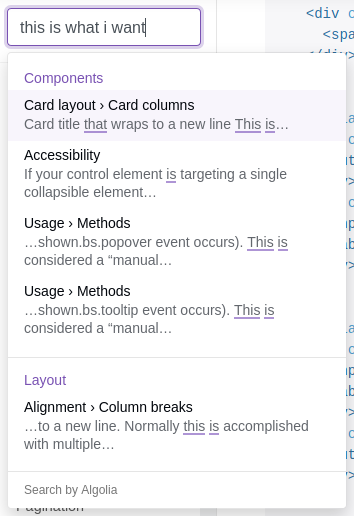
\includegraphics[scale=0.5]{searchresults.png}
    }
    \caption{What I wanted my search results to be like.}
    \label{fig:idealsearchresults}
\end{figure}

\subsection*{Solution}
To resolve this, I decided to redesign the website and place the search bar, instead of in the top right, instead in the centre, beneath starred subjects. It also becomes full-width that way. In theory, most users of the site wouldn't be accessing the full list of subjects often, so it shouldn't get in the way too much.

\subsubsection*{Commits}
\begin{description}\small
    \item[\texttt{230e87e}]  Added search functionality and moved bar to middle of screen
\end{description}

\begin{center}
\rule{0.5\textwidth}{0.2pt}
\end{center}

Adding the subjects page was basically copying bits of what I'd done from the first page, and rearranging them, while getting the parameters from the URL. From this point forward I actually had all the functionality complete, and was more working on improving the user experience, things to just make it a bit smoother, like adding a fade in on subject name due to the delay taken to find the name of the subject.

\section{User Feedback}
This feedback is mostly cumulative - for small improvements, I would make them as I went, and check them against future people. Larger improvements ended up in the improvements sections.
\subsection*{Elia}
\begin{itemize}
    \item He'd prefer, on the search results, the name of the subject to be listed. However, due to the fact that each standard can be associated with multiple subjects, this isn't possible (or at the very least, easy). 
    \item He would like starred standards that can be on a separate page. Organised by subject, easily accessible and fast loading.
\end{itemize}

\subsection*{Odin}
\begin{itemize}
    \item Centre-align the credits and levels, to properly associat ethem with their column.
    \item There are two of everything in Business Studies (I think this is because there's both ``Agribusiness'' and ``Business Studies'' that reference that subject, I fixed this by ignoring Business Studies). 
    \item Pressing enter on the search box breaks it, it goes to /? of the local thing. Searching on the subject page is also broken.
    \item Border between columns of standards as it gets confusing?
    \item Sort by different stuff (rather than just standard number) in list of standards.
\end{itemize}

\subsection*{Jasper}
\begin{itemize}
    \item Better distinction between search box and standards list to identify search box as global rather than just the standards listed below. Either that or make subject-specific search bar.
    \item Better distinction between internal and external standards, perhaps by a background colour change. Internal and external is an important distinction, maybe do internal first for each level, then external.
    \item Make level row unhoverable.
    \item He'd prefer if the search bar were not in the centre of the home page kinda randomly, maybe closer to the top.
    \item Mouse over a subject to get tooltip/dropdown of levels, which would go into URL parameters. Minimise scrolling. This could probably also be solved by starring standards per subject and listing those at the top of each subject.
    \item Make it more clear that you click the title in the top left to go back from the subject page. Maybe a ``home'' link in the navbar as well. Nav breadcrumbs (separated from logo) would also solve that. (e.g \texttt{Subjects > Chemistry})
    \item  Don't need whole-arse box with ``standards'' header for the list of standards. Maybe have a lighter-coloured background?
    \item Make starred subjects bigger, agrees with card idea. It would make it look more full, less samey-samey, and like there's more stuff going on. Use NCEA blue more, make cards interactive, with blue border on hover.
    \item Contact link to email, Github
\end{itemize}

\subsection*{Tim (my Dad, not you or Tim Hulbe-Pulver)}
\begin{itemize}
    \item Add ``New Zealand'' to header, to clarify
    \item Set people's expectations by mentioning only level 1-3, like ``New Zealand High School NCEA Subject Navigator''
    \item Add about page with short tech-description, why it was made etc.
    \item Short mantra e.g. `fastest way to find exams'
    \item Responsiveness shouldn't only be dependent on pixels wide (high res phones look bad)
    \item Update footer (add email)
    \item My Subjects? Favourite Subjects? Instead of ``Starred'', gives better idea of intention
\end{itemize}

\subsection*{Sarah}
\begin{itemize}
    \item External/Internal colour different shades of blue
    \item Red accents (underneath navbar)
    \item For subject-specific search, change placeholder text
    \item Font is wacky (Kiwi Maru), might be good to find a replacement like Roboto, also would make it consistent across browsers.
    \item A logo
    \item On iPhone, the buttons look bad.
\end{itemize}

\subsection*{Zishen}
\begin{itemize}
    \item Make name bigger (in top left)
    \item On chromebooks, the a tags look really bad, they look like default HTML buttons.
    \begin{itemize}
        \item This is apparently solved by \texttt{   -webkit-appearance: none;} on buttons and stuff, so I guess webkit doesn't override the CSS/SCSS from Bootstrap.
    \end{itemize}
    \item A bit confused by the colour of the external standards compared to the hover colour
    \item Other than that, it seems good. He's pretty happy with it.
\end{itemize}

\subsection*{Alex}
\begin{itemize}
    \item Change font for header (we chose Kiwi Maru), I will get other people's feedback on it
    \item On standards table, the hover is a bit extreme, maybe try to reduce it.
    \item Improve responsiveness, try developing on a higher-resolution monitor. Switch to media query on \textit{resolution} rather than how wide the screen is in pixels.
    \item Disable hover on mobile
    \item Could try more detailed background (like NZQA website) for navbar.
    \item Keep footer stuck at bottom to minimise jump when loading in standards on the subjects page
    \item For when there are no standards for a level of a subject, say ``no standards for level x'' and/or disable the link to that from the starred subjects page.
    \item Make header (subject name and ``Subjects'' text) unselectable
\end{itemize}

\subsection*{Paxton}
\begin{itemize}
    \item Search bar should be above My Subjects
    \item Other than that, it seems good. 
    \item He doesn't like the idea of Kiwi Maru for the header. Looks like OfficeMax, back to school vibe.
\end{itemize}

\subsection*{Mr Pirie}
\begin{itemize}
    \item Likes the website, hates the NZQA website.
    \item Might like a ``custom'' list of standards e.g. Level 1 Science + Level 2 Bio + Level 3 Bio
\end{itemize}
\subsection*{Mr Biggin}
\begin{itemize}
    \item Big improvement for him would be direct access to the achievement standards, so might as well go the whole way to individual exam papers. Then he could access the current achievement standard in a single click. Scraping would take a lot longer.
    \item As a half-way point, have a dropdown below each standard in the table that allows you to select \textit{only} exemplars, past papers, achivement standards, etc. like the middle dropdown in NZQA's NCEA search engine. \texttt{\&view=exams} URL parameter
    \item As well as this, maybe for each level a link to external papers, e.g. for science link to search results for the internal name of the subject with \texttt{\&view=exams} parameter.
    \item Add version column, or in dropdown beneath each standard with information like field, subfield, and domain.
    \item Starred standards
\end{itemize}

\section*{Short-Term Improvements}
\begin{itemize}
    \item \textbf{Aesthetic}
    \begin{itemize}
        \item These were all minor enough to be done during gathering of feedback
    \end{itemize}
    \item \textbf{Content}
    \begin{itemize}
        \item  Add an about page with more information about the reason it was made, a short tech-description about the components, and a bit about me. Link to github and contact details too.
        \item Breadcrumbs for navigation
        \item Analytics, home (subjects) and about pages could go in Nav bar to make it less empty
        \item Update footer with contact links
        \item Add short tag-line/quick description to tell people what it is.
        \item Organise subjects alphabetically
    \end{itemize}
    \item \textbf{Function}
    \begin{itemize}
        
        \item Dropdown beneath each standard in the table with:
        \begin{itemize}
            \item Big link to all NZQA documents for a standard
            \item Current version
            \item Field, subfield, domain (more breadcrumbs!)
            \item Link to \texttt{\&view=exams} (NZQA doesn't support this AFAIK, only for subjects)
            \item Link to current achivement/unit standard
        \end{itemize}
        \item Have buttons for each level (\texttt{\&level=<level>}) to take you to all the exams (\texttt{\&view=exams}), assessment specifications (\texttt{\&view=achievement}), and reports/schedules (\texttt{\&view=reports})
        \item \textbf{Literacy/Numeracy Credits} from NZQA, which for some gosh darn reason has a list of subjects that it associates with the standard. As well as this, it has proper accents on the titles and subjects finally. Only 866 standards are here though. Might require some ?, ? for each.
        \item Clear button on search box (for the text)
    \end{itemize}
    \item \textbf{Database}
    \begin{itemize}
        \item Re-map the internal name to the external name of a subject. Do this by having two name columns in the subjects table. Use the external name for basically everything, the internal name is only for scraping and redirection to the NZQA website. This could resolve issues surrounding  Te Reo M\={a}ori and Mathematics \& Statistics.
        \item Storage of the most recent achievement standard's year, or for unit standards, just a link to the unit standard
        \item Storage of the literacy/numeracy credit value.
    \end{itemize}
\end{itemize}

\section*{Long-Term Improvements}
\begin{itemize}
    \item Using starred standards and subjects, a ``My Year'' tab from the home page, where all information would be put together, with totals for literacy/numeracy/total credits, unit vs achieved etc.
    \item Direct access to NZQA documents on top of initial achivement standards (scrape each individual achievement standard page, as unit standards don't have documents)
    \item Allow sorting the standards table by various columns
    \item Custom content for advertisers
\end{itemize}

\begin{center}
\rule{0.5\textwidth}{0.2pt}
\end{center}

\section*{Challenges of Implementation}

\subsection*{About Page}
This was a bit tricky. I made a system diagram and short system description, but it looks really bad. This is going to be a progressive thing. Initially I have just gone with a description of the components involved in the system, and have also added a FAQ at the bottom for queries regarding things like \say{Why are there two columns in the literacy column?}

\subsection*{Display Names}
This is what I called storing both the internal and external name of subjects. This actually ended up working out really well, and worked near-flawlessly. Only a couple basic programming bugs regarding only implementing it in some parts of the website (e.g. Starred subjects showing internal name while the subjects list shows external name. 
\subsection*{Dropdowns}
This kind of broke everything. Bootstrap, the frontend library I am using, is really not designed for this. Bordered tables, padding, everything like that doesn't line up. There's a branch in the github repo that reflects this change, but it became a dead-end, I broke more than was worth it to fix. I am now planning to make a separate \texttt{/standard?num=91154} kind of page. So, I just worked on providing the literacy and numeracy information in the table, as this was a different feature requested by user testing. However...

\subsection*{NCEA vs UE Literacy and Numeracy}
Surprisingly, there are two separate definitions of literacy credits. \href{https://www.nzqa.govt.nz/qualifications-standards/awards/university-entrance/literacy-requirements/}{University Entrance}, and \href{https://www.nzqa.govt.nz/ncea/subjects/literacy-and-numeracy/level-1-requirements/lit-num-subjects/}{NCEA}. All standards that qualify for university entrance literacy qualify for NCEA, but not vice versa. The list of NCEA literacy standards hasn't been updated since April 2019, while the list of UE approved literacy standards is more regularly updated (last updated February 2020).

Numeracy credits are ambiguous, but I think what the website means is that the UE numeracy credits are the same as the NCEA numeracy credits. I have sent a question about this to the NZQA.

My solution for storing all this data, is removing literacy/numeracy as columns from the standards table, and adding two more tables:
\begin{itemize}
    \item \texttt{ue\_literacy} will contain \texttt{standard\_number} (FK), \texttt{reading} (bool), \texttt{writing} (bool)
    \item \texttt{ncea\_litnum} will contain \texttt{standard\_number} (FK), \texttt{literacy} (bool), and \texttt{numeracy} (bool)
\end{itemize}

I like this solution, as it separates all the different sources of information into separate tables. This means updating one doesn't mean updating them all. When retrieving the data through the Flask API, I will join the information together in a big ol' \texttt{JOIN} query, However, when putting this data in the Meilisearch database, I will stick it all together, so each standard has associated NCEA, UE literacy and numeracy booleans, in the same object, which can be served to the frontend directly.

%\begin{center}
%\rule{0.5\textwidth}{0.2pt}
%\section*{\texttt{v1.0}}
%\subsection*{Anything past this is more than the MVP (in my opinion)}
%\rule{0.5\textwidth}{0.2pt}
%\end{center}

\subsection*{Standard Page}
This will contain the information that would've initially gone in the dropdown. This is:
\begin{itemize}
    \item Big title, number
    \item Star button
    \item Link to all NZQA documents
    \item Current version (if known)
    \item Reading, writing, numeracy, NCEA literacy status.
    \item Subjects that are related (add an API endpoint for this, I can't associate every single standard with only a single subject)
    \item Field, subdomain, domain.
    \item Link to current achievement/unit standard
    \item Link to exemplars (this will be post the-big-scrape)
    \begin{itemize}
        \item Internals are at \texttt{nzqa.govt.nz/ncea/subjects/physics/annotated-exemplars/level-3-as91521/}
        \item While externals are PDFs.
    \end{itemize}
\end{itemize}

\subsection*{The Big Scrape}
The big scrape will be the scrape of every single `view-detailed' page for all the standards I have. This means I will have access to the full list of relevant documents, and can extract this information and put it in the database for serving from my website. This is a really big jump in functionality, hence `the big scrape'. As well as this, it'll be a lot of work, and require some smartness when it comes to putting things in the database. I want to retain simplicity and not over-complicate things to the point of obfuscation. I've also split it up into two stages. Stage 1 is scraping the \texttt{view-detailed} page, for the resources linked there, while Stage 2 is scraping the \texttt{annotated-exemplars} page, which will be a bit frustrating. I have two options for Stage 2. I can either scrape (and see if there's a 404) for each standard, or I can scrape the \textit{subject} annotated exemplars page, which contains links to all the annotated exemplars for each internal standard in the subject. The problem with this is that I only get the exact PDF URL from the specific standard page, but I'm pretty sure I can infer the PDF URL based on the standard URL.

The solution I ended up with was two tables --- a \texttt{resources} table, and a \texttt{resource\_categories} table. The \texttt{resource\_categories} table contains categories, for examples exams or exemplars, and has an associated category ID. The \texttt{resources} table contains information about the resource, and has foreign keys to the standard number and the ID of the category.

After Stage 1, there were a total of over 22 thousand overall resources that I added, and around 4.5k duplicates, for whatever reason. Most of these duplicates were subject-wide reviews, that were listed under nearly all of the standards within that subject (e.g. Technology review 2015 would be listed under the standards for wood tech, or metalwork, or anything like that.)

For Stage 2, I decided to use the solution of only scraping the pages for subjects, and handling any 404s I find. This worked out pretty well, and I think was quite an important change to make, because the annotated exemplars (although not intended for student eyes) are quite hard to reach if you don't know where to get them.

The schema that I had after the big scrape is shown in Figure~\ref{fig:scrapetp}
\begin{figure}
    \begin{center}
    \fbox{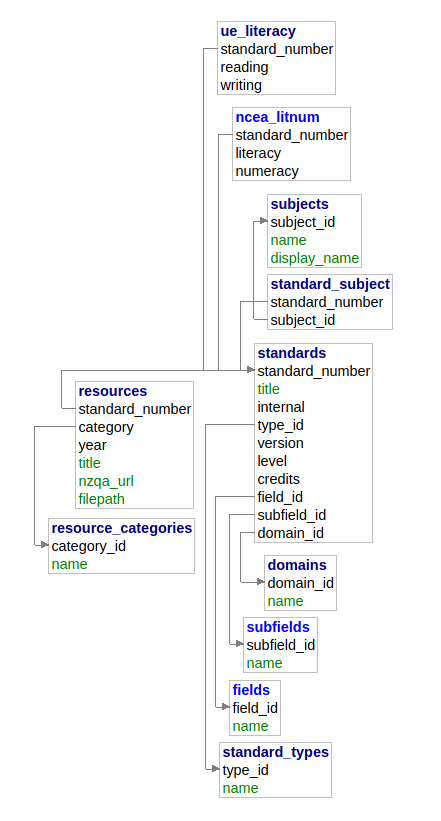
\includegraphics[width=0.4\textwidth]{post-scrape-db.png}}
    \caption{Database topography, post-scrape. Generated by Adminer.}
    \label{fig:scrapetp}
    \end{center}
\end{figure}

Adding the resources exaggerated the already present performance issues in my scraping script. It takes a couple minutes, which is more than it needs to. I could try porting to a faster language such as Rust. I have put this on an issue on Github as a potential future enhancement. I think it would be a good opportunity to use Rust, as it's a task that doesn't require user interaction, could be multithreaded (man that would be so cool), and doesn't use any special libraries. Meilisearch is written in Rust, so I'm sure there will be a cargo crate that I can import to interface with their database. As well as that, PostgreSQL is a very common enterprise database, so I'm confident there would be a nice crate interface. I would have to deal with strongly typed languages, but that's probably good, it would stop be from having so many errors.

\subsection*{My Standards}
This is basically the same as starred subjects, except for standards. This will also mean that there'll need to be a page for showing all of them, close to the home page. This page would show the total number of credits, UE literacy, numeracy, for each level etc. However, there's another complication...

\subsubsection*{Exclusions}
\href{https://www.nzqa.govt.nz/qualifications-standards/standards/standards-exclusion-list/}{Exclusions!} These happen when there are two standards (one unit, one achievement) where the standards assess similar things. The NZQA manages a list of these conflicts, and decides which one the credits should be given for, if both are assessed. This will be important to implement with my ``My Year'' tab thing, I could highlight exclusions if they do come up, however this is going to be one heck of an edge case, as I'm confident schools will already manage this sort of thing and ensure conflicts/exclusions do not occur.

I will store all this data in an \texttt{exclusions} table, with a \texttt{preferred} column, and an \texttt{excluded} column. These columns will contain standard numbers. In the case of an exclusion/conflict, the credits from the \texttt{preferred} standard will be given.

This could be used in two ways. Either, I could have the backend do the calculations, given a list of standard numbers, the totals for literacy/numeracy, by accounting for exclusions, or I could have the frontend take all exclusions and do the calculations. Doing it on the frontend would increase the efficiency of caching, but backend calculation could be faster, because SQL be speedy. There are $\sim1620$ exclusions, so I might do this on the backend.

Later down the line, I thought more about whether it was worth it to implement these exclusions. I decided it wasn't worth it, and instead decided to just put it in the FAQ, as if people ask me that question. The chances that such a thing would show up are extremely limited, as the institutions are a part of would almost certainly already check this sort of thing with the software they use (e.g. Edge).

If anyone explicitly requests exclusions to be implemented, I will do that.

\subsection*{Custom Content}
The ability to modify the content beneath each subject title and each level in a given subject was more useful than I initially thought. It allows the user to have access to a curated list of study resources relevant to the subject and level. Implementation involved an extra database table, \texttt{custom\_content} which contained \texttt{subject\_id}, \texttt{level}, and \texttt{html}. This was updated through JSON files with the format:

\begin{verbatim}
{
    "content": [
        {
            "subject": <subject_id>
            "general": ["<html to go at top of page>"],
            "level_1": ["<html to go below level 1 header>"],
            "level_2": ...
        },
        {
            "subject": <subject_id>
            ...
        }
    ]
}
\end{verbatim}

Multiple files of this format could be created, and stored in the \texttt{scrape/content/} directory. The \texttt{scrape} container would then look through all files in that directory and extract the information, collate it into a format that could be stored in the database.

The API would then access this information stored in the database and serve it upon request to the \texttt{/api/content?id=<subject\_id>} endpoint. The frontend then displays this information where it should go.

In order to modify the content and then refresh the database from the new JSON files, I had to get the scraping script to know when I wanted it to be refreshed. I did this by adding a \texttt{flags} table in the database that could store information for when I wanted the database to update. I didn't create any API endpoints that would modify this, but I instead created a Bash script that allows me to directly run a command onto the PostgreSQL container. It's a bit disgusting, but it kind of makes sense:

\begin{verbatim}
docker-compose exec db psql -U nzqa -c "INSERT INTO flags (name) VALUES '$1';"
\end{verbatim}

The first segment (\texttt{docker-compose exec db}) tells docker compose to run the following command on the \texttt{db} instance. The command runs the \texttt{psql} script which allows command-line interfacing with the postgreSQL database running in that container. The \texttt{-U} flag tells \texttt{psql} to use the database \texttt{nzqa}, while the \texttt{-c} flag contains the actual SQL query to execute.

\section{Other considerations}

\subsection*{Accessibility}
The Bootstrap docs have helpful tips about how to keep the site accessible, using \texttt{aria-} data attributes for screenreaders. Hence, I've used them around my site. My brother (because he felt like it) tried to use the site without a mouse, tabbing around to all the links, and it worked quite well. From this point forward, I made sure that I was adding \texttt{aria-} attributes where appropriate and necessary.

\subsection*{SEO}
I've never done search engine optimisation before, but I got myself registered for the Google search console, and requested indexing on my site. The indexed site's titles are not exactly the same as the \texttt{<title>} tag, so some optimisation was required there.

After indexing the site, I made sure that the \texttt{meta} tags contained adequate descriptions of things, and that the titles were roughly what you'd want to Google. Thankfully, Google runs the Javascript on pages that it indexes, so I could update the title of a standard or subject page after I'd requested that kind of information from my server.

A month after initially indexing the site, I found that I had already made 5000 `impressions', which is what Google calls `showing up in search results'. I think this indicates that my SEO worked, and that my target audience (those searching for the NZQA website) was seeing my website in their search results. However, (nearly) nobody clicked on it, so my CTR (click-through rate) was only 1.8\%. My average position in search results was 6.8, which I think is pretty good, considering very few people would be explicitly searching for my website. Google shows the top 10 search results on the first page as far as I know, so there's a good chance people have seen it.

\newpage

\section{Relevant Implications}
In a project such as this, where I am building a product that has real-world use, it has been more important than ever to consider the implications of the work I do. Failure to do so could cause problems for potential users and myself, and could harm the product's functionality and use, or leave myself open to legal problems.

\subsection*{Legal}
Running a service that serves content created and curated by other people is inherently questionable from a copyright standpoint, so required some investigation. Luckily, I didn't have to look too far. The NZQA website explicitly outlines their policy on their resources. This happens to have an exception for ``Internet sites wishing to link to NZQA websites'' (that's me!) where they say:

\begin{quote}
Internet sites may link to NZQA websites or material on it, and use the NZQA logo in doing so. However, only the following statement about NZQA may be made when referring to NZQA:
    
    \begin{quote}
    ``The New Zealand Qualifications Authority ensures that New Zealand qualifications are valued as credible and robust, both nationally and internationally.
    
    NZQA is accountable for:
    \begin{itemize}
        \item managing the New Zealand Qualifications Framework,
        \item administering the secondary school assessment system,
        \item independent quality assurance of non-university education providers,
        \item qualifications recognition,
        \item standard setting for some specified unit standards, and
        \item the development of qualifications in specific fields.''
    \end{itemize}
    \end{quote}
\end{quote}

So, from this, I can see that I can either say nothing, or specifically that thing about NZQA. I chose to say nothing, as it's just easier, and I don't have much reason to say anything about them. As well as this, my use of their logo in my about page is also legal. I am not claiming the content, and often explicitly mention where the content comes from, so I reckon that I'm pretty well in the clear on that front.

In terms of resources that are ``Crown Copyrighted'', the rules are, according to the Intellectual Property Office of New Zealand:
\begin{quote}
    \begin{itemize}
        \item Content from Crown publications and web pages can be copied, accessed, viewed, reproduced and printed for non-commercial purposes. You should credit the owner (e.g. Ministry of Business, Innovation \& Employment or IPONZ) and source (e.g. ISBN, ISSN, ISMN or web page address).
        \item All Crown information must be accurately reproduced, and exclude anything that has been officially redacted/blacked out.
        \item You must not use the material in a manner that is offensive, deceptive or misleading.
        \item You should contact the government ministry, agency or state-owned enterprise concerned for clearance to reproduce and recoup copying costs or re-use protected Crown copyright works. You will need permission if you intend to on-sell government information from public records and government information. You must have authorisation to use a New Zealand government logo or emblem.
    \end{itemize}
\end{quote}

I believe I am in the clear in this way. I credit the source of the content in the name of my website ``\textbf{NCEA} Subject Navigator'', and I put a disclaimer on the about page, saying that the resources I serve are under Crown copyright and produced by the NZQA.

\subsection*{Functionality}
Functionality is an essential consideration for the production of any digital outcome. In a large-scale (by my standards) project, such as this, it is even more important. Creating a product that performs as well as possible ensures that it can be used effectively by everyone. There were a large number of times during the development of NSN in which I had to make decisions to ensure the functionality of the final outcome.

The decisions I made during the creation of the scraping script(s) (under \texttt{/scrape/code/}) were made quite early on --- when I still wasn't entirely sure how the final product would fit together. However, there were a variety of features and functionality I added to try to keep my options open and ensure that the script itself worked as well as possible. These included:
\begin{itemize}
    \item Caching the retrieved content from the NZQA website as files, and retrieving them when necessary
    \item Adding in a random delay between requests of around 5-10 seconds. This was necessary because I think aafter some time NZQA started rate-limiting me for my repeated, periodic requests. This randomness ``simulated" a human navigating their website, and hopefully wouldn't trigger DoS detection.
    \item Automatically scraping (or at least checking) every 6 hours whether something has to be done, whether this be updating the database from the cached information, or fully rescraping.
    \item Using a simple JSON interface for modification of the custom content, and allowing for multiple JSON files to be made, which allows me to organise the custom content by provider, without ending up with a uselessly large comment-less (JSON doesn't allow comments) file.
\end{itemize}

In a whole-project sense, the movement to Docker containerisation and coordination with \texttt{docker-compose} was a significant step that increased functionality hugely. It meant that I could easily migrate to multiple different machines (basically all it needed was \texttt{docker-compose up} on the new machine), and didn't have to worry about dependency issues happening between the two Python scripts I had to keep running (scraping/DB management + the API service), because they were in separate containers. It increased security, as there were hard limits as to what could be accessed from the outside, and this turned out to just be the Caddy container. The Caddy container then directed traffic to where it needed to be, whether that be Meilisearch, GoAccess, my API, or serving static files. Speaking of Caddy, Meilisearch, and GoAccess, the implementation of these drop-in components of NSN was trivial. This is particularly well-exemplified by the implementation of Meilisearch, which was three lines in my \texttt{docker-compose.yml}:
\begin{verbatim}
search:
    image: getmeili/meilisearch:latest
    restart: unless-stopped
\end{verbatim}
GoAccess and Caddy were a bit of a different story, where I had to configure volumes that the container could access on the host system, which allowed for persistent SSL certificates (it felt really bad to be rate-limited by LetsEncrypt before I'd implemented that persistence), and sharing the Caddy logs to the GoAccess container for parsing and display. However many troubles I encountered trying to configure the volume sharing was far outweighed by the ability Docker gave me to incredibly simply add new packages to my project, without making it harder to migrate to another platform. Another such package that I found invaluable was Adminer, which was another very small addition to my \texttt{docker-compose.yml}:
\begin{verbatim}
adminer:
    image: adminer
    restart: unless-stopped
    ports:
        - 8080:8080
\end{verbatim}
Adminer allowed me to have a quick, easy interface with the database. This proved invaluable when troubleshooting errors in my API, and to see for example whether it was right about information not being there. It also meant I could test SQL queries in a far easier way than the \texttt{psql} Bash interface which is a real pain to use.

Overall, Docker gave me the ability to far improve the functionality of the whole project, as it expanded the scope of possible extra packages I could use, which I would have otherwise not used for fear of worsening migration cost/energy.

\subsection*{End-user Considerations}
The end-user was constantly the focus for the foundational decisions made
\begin{itemize}
    \item Linking to resources is super beneficial from a user standpoint
    \item Took user feedback (Mr Biggin) and implemented viewing of the most current version of each standard
    \item Sharing lists of standards allows course designers to preview their course, and teachers to share a course and relevant resources with their students
    \item Being very selective in what study resources I link to means that every link counts, and that people will pay attention to everything
    \item Linking directly to PDFs rather than to standard pages for NZQA improves response time (I don't have to go through their search engine, which is slow on repeated queries)
    \item Not just listing all resources, I organise them by category
    \item Linking to annotated exemplars, which are hard to find
\end{itemize}


\subsection*{Privacy}
\begin{itemize}
    \item Don't store any data
    \item Actively try to prevent access to data (removing IP from GoAccess dashboard, hiding logs)
\end{itemize}

\subsection*{Future Proofing}
\begin{itemize}
    \item Good documentation, a writeup, using accurate git commits, and versioning with github tags + releases. 
    \item Expandable database format, with constant dynamicism with the scraping script, allows for great flexability.
    \item Anticipation of the upcoming change to NCEA
    \begin{itemize}
        \item Everyone I've talked to has said that things will still be organised as standards with resources, and the NZQA website format should still be okay, so a re-scrape won't create too much of a hazard to functionality.
    \end{itemize}
\end{itemize}

\subsection*{Accessibility}
\begin{itemize}
    \item \texttt{aria-} tags for labels and purposes
    \item Alt-texts for all images
    \item Text-based normal \texttt{<a>} tag navigation means that it's quite easily navigable for screen-readers and non-graphical interfaces (as long as they run Javascript)
\end{itemize}

\end{document}
